\section{System identification by noise excitation}
\subsection{Cross-correlation method:}
In the discrete domain we have the normalised cross-correlation of two signals \(x\) and \(y\):
\begin{equation}
	\gamma_{xy}[m] = \frac{1}{L}\sum_{n=-\infty}^{\infty} x[n]y[n+m]
	\label{eq:crossdef}
\end{equation}
Where \(L\) is the length of the two signals combined. The special case of auto-correlation emerges when \(x=y\). 

When \(y\) is the product of convolving (filtering) \(x\) with an impulse response \(h\), eq.~\ref{eq:crossdef} becomes
\begin{equation*}
	\gamma_{xy}[m] = \frac{1}{L}\sum_{n=-\infty}^{\infty}x[n]\sum_{k=-\infty}^\infty x[n+m-k]h[k]
\end{equation*}
Which reduces to the convolution of the auto-correlation of \(x\) with \(h\)
\begin{equation*}
	\gamma_{xy}[m] = \frac{1}{L}\sum_{k=-\infty}^\infty \gamma_{xx}[m-k]h[k]
\end{equation*}
Meaning that the cross-correlation of a signal and a filtered version of itself is equal to the filtered auto-correlation. 
For a white noise signal \(x\) of infinite length we know that \(\gamma_{xx}[m]=0\, \forall\, m\neq 0\) and \(\gamma_{xx}[0]=1\).
Therefore the cross-correlation of a white noise signal and itself filtered with an impulse response \(h\) can be reduced to
\begin{equation*}
	\gamma_{xy}[m] = h[m]
\end{equation*}

Applying this result to the given input/output pairs we obtain a very long impulse response. This is because we are actually 
performed convolution and so the length
of the obtained impulse response is \(m+n-1\) where \(m\) and \(n\) are the lengths of the input and output respectively.
However, by visual inspection of the resulting signal, it is clear that the amplitude of the impulse response obtained from
corss-correlation becomes 
insignificant after approximately 200 samples, starting from a lag of 0. We therefore apply a rectangular window starting at
lag 0 and extending 200 samples for all signals, except the input/output pair of length 100 that only have 100 samples starting
from lag 0. For this signal we use a rectangular window of 100 samples.

The resulting impulse responses and the estimates frequency response of the system can be seen in figures~\ref{fig:xcorr_IR} and~\ref{fig:xcorr_freqz} respectively.

\begin{figure}
	\center
	\includegraphics{./picture/xcorr_IR.eps}
	\caption{Impulse responses obtained by cross-correlating the input/output pairs. Legend shows number of samples in
	input/output pair.}
	\label{fig:xcorr_IR}
\end{figure}

\begin{figure}
	\center
	\includegraphics{./picture/xcorr_responses.eps}
	\caption{Frequency responses of the impulse responses obtained by cross-correlation. The system is clearly a bandpass filter 
	passing through normalised frequencies around 0.2.}
	\label{fig:xcorr_freqz}
\end{figure}

\begin{figure}
	\center
	\includegraphics{./picture/rconv_IR.eps}
	\caption{Impulse responses obtained by reserve convolving the input/output pairs. Legend shows number of samples in input/output pair.}
	\label{fig:rconv_IR}
\end{figure}

\begin{figure}
	\center
	\includegraphics{./picture/rconv_responses.eps}
	\caption{Frequency responses of the impulse responses obtained by reverse convolution. These responses agree with the ones obtained
	by cross-correlation. The system again seems to be a bandpass filter accepting normalised frequencies around 0.2.}
	\label{fig:rconv_freqz}
\end{figure}

\subsection{Reverse convolution method:}
We should be able to reach the same result by reverse convolution since the processed noise output is just the input convolved with
the impulse response of the system. Let \(h\) be the system impulse reponse, \(x\) the input and \(y\) the output. In the 
frequency domain, convolution is simple multiplication and therefore finding the transfer function, the fourier transform of the system impulse
response is simply:
\begin{equation*}
	h=\frac{y}{x}
\end{equation*}
The results of this analysis can be seen in figures~\ref{fig:rconv_IR} and~\ref{fig:rconv_freqz}.
